\documentclass[tikz,border=5pt]{standalone}
\begin{document}
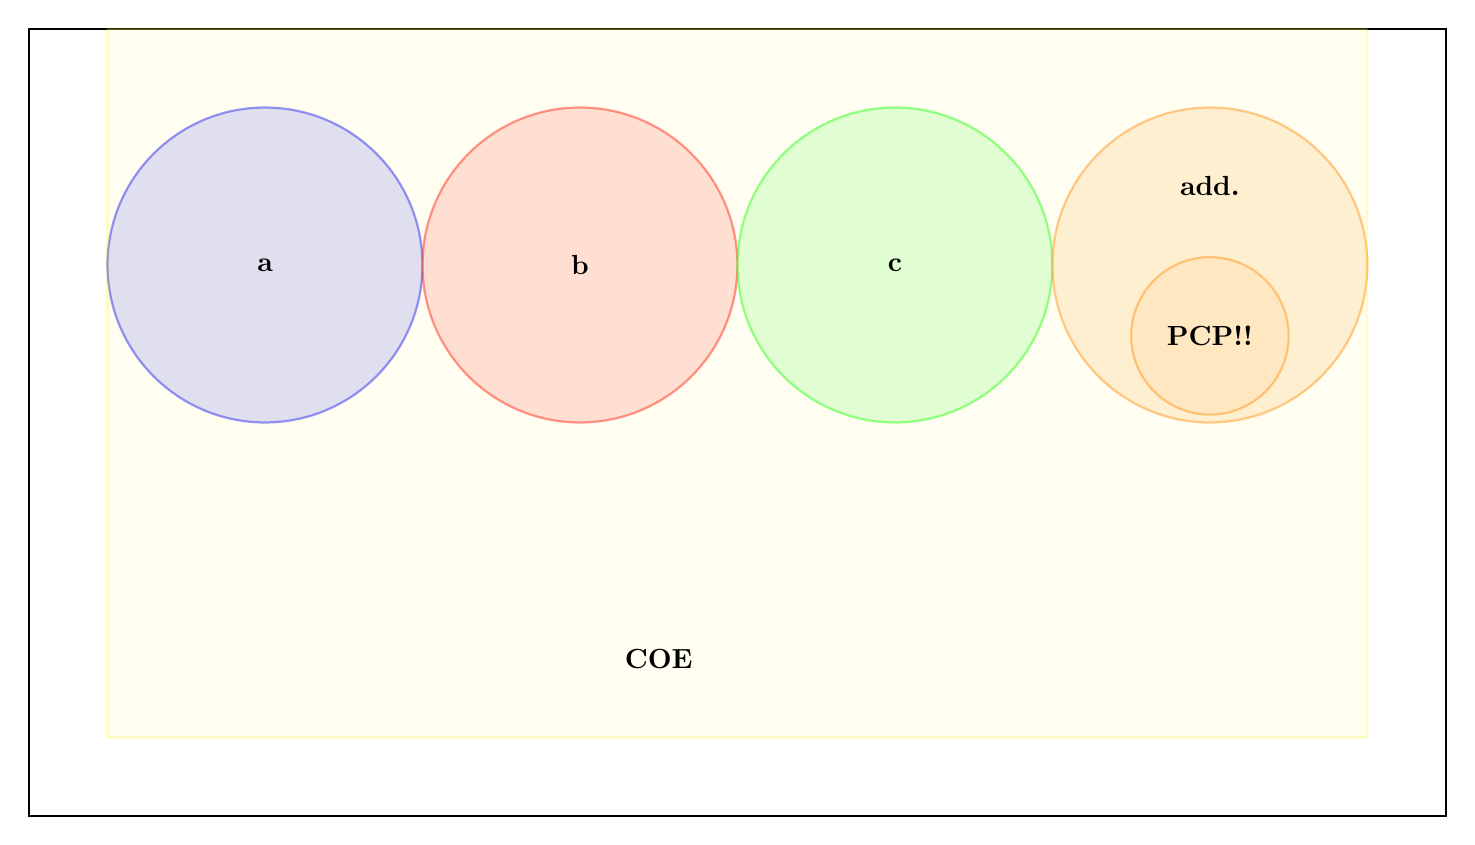
\begin{tikzpicture}
    % Draw the large box
    \draw[thick] (0,0) rectangle (18,10);
    
    % Draw four circles for the Venn diagram
    % Top left circle
    \draw[fill=blue!30, opacity=0.5, draw=blue, thick] (3,7) circle (2);
    
    % Top right circle
    \draw[fill=red!30, opacity=0.5, draw=red, thick] (7,7) circle (2);
    
    % Bottom left circle
    \draw[fill=green!30, opacity=0.5, draw=green, thick] (11,7) circle (2);
    \draw[fill=orange!30, opacity=0.5, draw=orange, thick] (15,7) circle (2);
    \draw[fill=orange!30, opacity=0.5, draw=orange, thick] (15,6.1) circle (1);
    
    % Bottom right circle
    \draw[fill=yellow!30, opacity=0.2, draw=yellow, thick] (1,1) rectangle (17,10);
    
    % Add text in the center of the diagram
    \node at (8,2) {\textbf{COE}};
    \node at (3,7) {\textbf{a}};
    \node at (7,7) {\textbf{b}};
    \node at (11,7) {\textbf{c}};
    \node at (15,8) {\textbf{add.}};
    \node at (15,6.1) {\textbf{PCP!!}};



\end{tikzpicture}
\end{document}